\documentclass[a4paper]{ltjsarticle}

\usepackage[deluxe,noto-otf,no-math]{luatexja-preset}
\usepackage{luatexja-otf}
\usepackage{graphicx}
\usepackage{listings}
\usepackage{amssymb,amsmath} %数式環境
\usepackage{siunitx} %SI単位系の出力
\usepackage{here}
\usepackage{tikz}
\usepackage[margin=0.8in]{geometry}

\setmainfont[BoldFont=Noto Serif CJK JP Bold]{Noto Serif CJK JP Regular}
\setsansfont[BoldFont=Noto Sans CJK JP Bold]{Noto Sans CJK JP Regular}

\topmargin = -10truemm
\headheight = 0pt
\headsep = 0pt
% \textheight = 250truemm

\setcounter{tocdepth}{3}

\title{第4回輪講補講資料 \\ 「コンピュータネットワーク」 \\ 第2章 物理層(pp.101-115)}
\author{岡崎 雅大 <Masahiro Okazaki> \\ okazaki@nile.cse.kyutech.ac.jp}
\date{2019年5月13日(火)}

\begin{document}
\maketitle
\tableofcontents

\section{より対線}\label{ux3088ux308aux5bfeux7dda}

\subsection{構造}\label{ux69cbux9020}

1mm程度の太さの2本の絶縁された銅線をらせん状により合わせて作られる.
一般にはよられた4対8芯の線が,線を保護し,一緒に保守するためプラスチックのさやにまとめられている.
また,それぞれの芯は1本の銅線で構成される単線,または7本の細い銅線で構成されるより線の2種類がある.
単線はノイズの影響を受けにくいが,ケーブルが固くなるため取り扱いにくくなる.
より線はノイズの影響を受けやすい一方,ケーブルが柔らかいので折り曲げて使用するような用途に向いている.

\subsection{伝送手法}\label{ux4f1dux9001ux624bux6cd5}

\subsubsection{差動モード伝送}\label{ux5deeux52d5ux30e2ux30fcux30c9ux4f1dux9001}

より対線では1対のより線単位で通信を行う.
2本の信号線のうち1本にプラスの電圧をかけ,もう1本にはマイナスの電圧をかける.
受信側では2本の信号線の差分を検出し,差がないときは0,差があるときは1と判断する.
これを \textgt{\textbf{差動モード伝送}} という.
差分を取ることによって,送受信間において基準電位を合わせる必要はなく,基準電位がずれていても問題にはならない.
さらに外部雑音に対しても良い影響を与える.

\subsubsection{信号線の組}\label{ux4fe1ux53f7ux7ddaux306eux7d44}

Ethernetの規格によって,4対ある信号線をどのように使用するかが異なっている.

\begin{itemize}
\item
  100BASE-TX以下 : \\
  4対の信号線を2対のみを用い,残りの2対は使用しない.それぞれのうち一方を送信用,もう一方を受信用として使い分けている.
\item
  1000BASE-TX : \\
  4対の信号線を2対ずつ送信用と受信用に分けて使用する.
\item
  1000BASE-T以上 : \\
  4対の信号線のそれぞれを送信用,受信用ともに使用する.信号が双方向に流れるため,送信と受信の信号を分離するためのハイブリッド回路と呼ばれる特殊な回路が必要になる.
\end{itemize}

\begin{figure}[H]
  \centering
  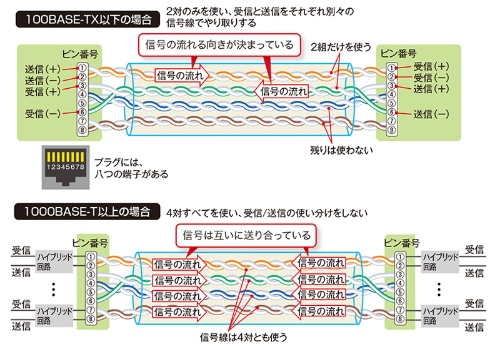
\includegraphics[width=10cm]{twistpair_system.jpg}
  \caption{信号線の使用方法\cite{2}}
\end{figure}

\subsection{カテゴリによる区別}\label{ux30abux30c6ux30b4ux30eaux306bux3088ux308bux533aux5225}

より対線による配線にはいくつかの種類がある.
それらはカテゴリとして規定されており,それぞれにおいて伝送帯域と対応するEthernetの規格が規定されている.
また,それぞれのカテゴリは下位互換性を有している. 
カテゴリを以下の表1に示す.

\begin{table}[H]
  \centering
  \caption{LANケーブルのカテゴリ}
  \begin{tabular}{c|c|c|c}
    カテゴリ & 伝送速度 & 伝送帯域 & 規格 \\ \hline
    CAT1 & 20kbps & - & \\
    CAT2 & 4Mbps & \SI{1}{MHz} & \\
    CAT3 & 10Mbps & \SI{16}{MHz} & 10BASE-T\\
    CAT4 & 16Mbps & \SI{20}{MHz} & \\
    CAT5 & 100Mbps & \SI{100}{MHz} & 100BASE-TX\\
    CAT5e & 1Gbps & \SI{100}{MHz} & 1000BASE-T\\
    CAT6 & 1Gbps & \SI{250}{MHz} & 1000BASE-TX\\
    CAT6a & 10Gbps & \SI{500}{MHz} & 10GBASE-T\\
    CAT7 & 10Gbps & \SI{600}{MHz} & 10GBASE-T\\
    CAT7a & 10Gbps & \SI{1000}{MHz} & 10GBASE-T\\
    CAT8 & 40Gbps & \SI{2000}{MHz} & 40GBASE-T\\
  \end{tabular}
\end{table}

\subsection{シールドによる区別}\label{ux30b7ux30fcux30ebux30c9ux306bux3088ux308bux533aux5225}

\subsubsection{UTP(Unshielded Twisted
Pair)}\label{utpunshielded-twisted-pair}

単に導線と絶縁体で構成されている配線形式のことを
\textgt{\textbf{非シールドより対線 (Unshielded Twisted Pair : UTP)}} という.
しかし,ノイズの影響を低減させ伝送帯域を増加させるために4つのより対線を仕切るように十字の構造物を含むUTPケーブルも存在する.

\subsubsection{STP(Shielded Twisted
Pair)}\label{stpshielded-twisted-pair}

個々のより対および,ケーブル全体の周りにシールドを有するケーブルのことを
\textgt{\textbf{シールドより対線 (Shielded Twisted Pair : STP)}} という.
規格としてはSTPではなく, \textgt{\textbf{FTP (Foil Twisted Pair)}}
と規定されている.
また,FTPが規定されているのはカテゴリ7からであり,それ以前のFTPケーブルについては各メーカーの独自実装である.
シールドによって,より対線自身から輻射されるノイズの抑制に効果がある.
しかし,シールドの接地を取らなければシールド自体が伝導体となってノイズの発生源となる可能性があるため注意が必要である.

\begin{figure}[H]
  \centering
  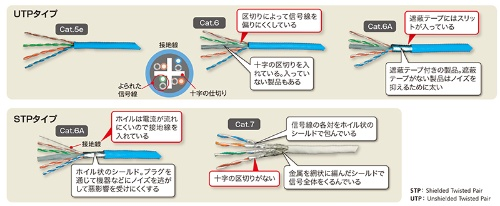
\includegraphics[width=10cm]{lancable.jpg}
  \caption{LANケーブルの例\cite{2}}
\end{figure}

\subsection{ノイズ対策}\label{ux30ceux30a4ux30baux5bfeux7b56}

\subsubsection{内部雑音}\label{ux5185ux90e8ux96d1ux97f3}

内部雑音としては \textgt{\textbf{漏話(クロストーク)}} が挙げられる.
ここで漏話とは,他の銅線に流れる信号波形による干渉を受けて本来の信号波形が乱されることを指す.
漏話は銅線に信号が流れるときに発生する磁束線によって発生するため,個々の銅線に対するシールドが効果を発揮する.
シールドによって銅線から発生する磁束線が減少する.
また,銅線をより合わせることでより対線を流れる信号によって発生する磁束は隣のより同士で反転しているため,お互いに打ち消し合う.
さらによりの数を増やすことによって打ち消し合う効果は大きくなっていく.
よって,カテゴリ5はカテゴリ3と比較してメートルあたりのよりの数を増やしている.
これらによって漏話の発生を抑えることができる.
また,隣の対との近さによっても影響の度合いは変化するため,ケーブル内においてより対線が密着しづらいようにゆったりめの構造にしたり,十字の仕切りを入れたりしている.

\subsubsection{外部雑音}\label{ux5916ux90e8ux96d1ux97f3}

外部雑音は差動モード伝送とよりによって低減させる.
差動モードでは1対の信号線のそれぞれにプラスの電圧とマイナスの電圧をかけて伝送し,受信側では信号線の差分を検出して信号を取り出す.
外部雑音は1対の信号線のそれぞれに同様に影響を与えることが多い(コモンモード・ノイズという)ため,差分を検出することでノイズの影響を無視することができる.
また,銅線をよることでよりを貫通する磁束により発生する電流は隣のより同士で反転しているため,互いに打ち消し合う.

\begin{figure}[H]
  \centering
  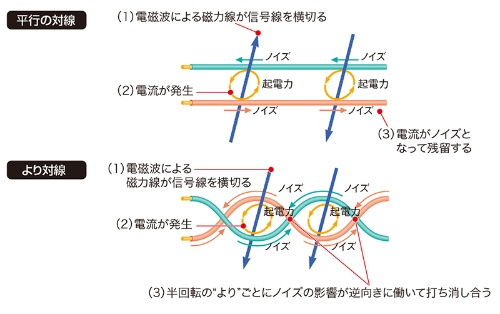
\includegraphics[width=10cm]{out_noise.jpg}
  \caption{よりによる外部雑音の低減\cite{2}}
\end{figure}

\begin{thebibliography}{9}
  \bibitem{1} コネクタ\&ケーブル(2),より対線と光ファイバが主流,https://tech.nikkeibp.co.jp/it/article/COLUMN/20060725/244199/,2019年5月13日閲覧
  \bibitem{2} LANケーブルの正しい使い方,https://tech.nikkeibp.co.jp/it/atcl/column/17/012300631/,2019年5月13日閲覧
  \bibitem{3} 100Base-TX、1000Base-TX、1000Base-Tにおける伝送方式の違い,http://www.aim-ele.co.jp/tech/metal-tech6/,2019年5月13日閲覧
  \bibitem{4} より対線ってなんですか,https://tech.nikkeibp.co.jp/it/article/COLUMN/20060530/239398/,2019年5月13日閲覧
\end{thebibliography}

\end{document}
